\documentclass[../main.tex]{subfiles}
\begin{document}
\subsection{Условие применимости метода линеаризации в задаче локального синтеза} 
We consider the problem of a feedback control design for a nonlinear control-affine system. The aim of the control is to bring  trajectories of the closed system to the origin of coordinates in a given time, providing the minimal value of an integral functional. The object under study is the nonlinear system, closed by a linear feedback controller. The controller is  obtained as a solution of the LQR problem for the linearized system. We indicate sufficient conditions  for this linear feedback to give a local solution to the control synthesis problem under consideration.  In addition, we give some  error estimates for the values of the functional. 

\subsection{Introduction}

We propose here a method for solving the problem of a local control synthesis  for a control-affine system on a small time interval. This method is based  on the linearization of the original nonlinear system in the vicinity  of the equilibrium position.  Linearization is often used in solving various control problems, such as stabilization problems\cite{Kras_add,Khalil}, stochastic and numerical control\cite{Roxin,EKF,denBerg,Pang}, MPC control\cite{Murillo,LTV_MPC}, etc.

In this article, we study the problem of control synthesis with an integral quadratic cost. Note that the task is considered on a finite, and, moreover, small, time interval. The goal of the control is to transfer the system to the origin in a given time ensuring the minimum value of the cost. The linear feedback control found for the linearized system is used as  the input of the original non-linear system. For a linear control system the optimal feedback is linear in state, with gains increasing indefinitely when approaching the terminal time. The latter  makes it difficult to justify the applicability of the linearization method. The restrictions on  asymptotics  of the controllability Gramian of the linearized system are needed in this case. Unlike, for example, the stabilization problem for which controllability (stabilizability) of the linearized system implies stabilizability of the nonlinear system. These restrictions coincide with the  asymptotic equivalence conditions for reachable  (null-controllable) sets of nonlinear and linearized systems. In \cite{GusevOsipov} it was shown that, under these conditions the control in the form of a linear state feedback takes all trajectories starting from some neighborhood of zero to zero, if the control time interval is sufficiently small. 

In this article, we generalize the main result of \cite{GusevOsipov}. The proposed sufficient conditions have the form of an inequality for some improper integral. They depend on the smallest and the largest eigenvalues of the controllability Gramian of the linearized system and contain a scalar parameter. The choice of this parameter makes it possible to cover a wider class of control systems, the conditions from \cite{GusevOsipov} are obtained here as a special case for a certain value of the parameter.

For a linearized system, the considered linear controller delivers the minimum value to the integral functional for any initial state. For a nonlinear system, this is not the case, so it is important to obtain an estimate of the resulting error. This was done in the second part of the article, where  the relation between the values of the integral cost for the trajectories of the nonlinear and linearized systems was studied and  the estimate for the relative error was given. 

The article is structured as follows. The problem statement and some preliminary results are given in the second section. The third section contains the formulation and proof of the main results. Finally, we provide two illustrative examples in the fourth section.

\subsection{Preliminary results}
\subsubsection{Problem statement}

Let us consider the nonlinear  control-affine system
\begin{gather}\label{sec22:nonlinear}
	\dot{z}(t)=f(z(t))+B u(t),\qquad 0 \leqslant t \leqslant T, \qquad z(0) = z_0.
\end{gather}
 where $ x \in \mathbb{R}^n $ is a state vector, $ u \in \mathbb{R}^r $ is a control vector,  $ 
T$ is a positive number. We postulate that the function $f$ has the following property. 
\begin{property}\label{prop:Residial_term_bounds}
	 There exist  $r>0$, $k>0$  such that for all $ z \in B(0,r) $ the function $f(z)$ could be rewritten in the form $ f(z) = Az + R(z) $, where  $ \|R(z) \| \leqslant k \| z\|^2  $. 
\end{property}
Here $ B(0,r) $ is the ball of radius $r$  centered at $0 \in \mathbb{R}^n$. 
This property holds if $f(0) = 0 $, $\frac{\partial f}{\partial x}(0) 
= A $ and $f(z)$ is twice differentiable. 

The space of square integrable scalar or vector functions on $ [0,T] $ we will denote by $ \mathbb{L}_2 = \mathbb{L}_2[0,T] $. The ball in the space $\mathbb{L}_2$ we denote as $B_{\mathbb{L}_2}(0,r)$. As the cost functional we consider the following
\begin{gather}\label{cost}
		I(T,u):=\int_0^Tu^\top (t)u(t)dt= 	\lVert u(\cdot)\rVert^2_{\mathbb{L}_2.} 
\end{gather}
The problem is to synthesize a feedback control $u(t)=u(t,z(t))$ that leads the trajectories of the closed system 
\begin{gather*}
	\dot{z}(t)=f(z(t))+B u(t,z(t)),\qquad 0 \leqslant t \leqslant T, \qquad z(0) = z_0.
\end{gather*}
to the origin of coordinates at  time $T$ and to provide the minimum value of $I(T,u)$. 

Consider the linear case ($R(z)=0$)
\begin{gather}\label{sec22:linear}
	\dot{z} =  A  z + B u, \qquad 0 \leqslant t \leqslant T.
\end{gather}
If  system (\ref{sec22:linear}) is controllable the solution of the above problem  is the linear in state feedback controller 
\begin{gather}\label{linear_feedback}
	u(t,z) = -B^{\top} Q_T(t) z
\end{gather}
(see, for example, \cite{Abgar,Kur1,GusevOsipov}).
Here $Q_T(t)=W^{-1}(T-t)$ where $W(t)$ is the Controllability Gramian of system $\dot{x} = -A x - B u$:
\begin{gather*}
    W(t) = \int_0^t e^{-A\tau}BB^\top e^{-A^{\top}\tau}d\tau. 
\end{gather*}
The Gramian $W(t)$ is positive definite for $t>0$ iff  
system (\ref{sec22:linear}) is controllable. It may be shown that $Q_T(t)$ is the solution of differential equation 
\begin{gather}\label{eqQ}
	\dot{Q_T}  = Q_T B B^{\top} Q_T - A^{\top}Q_T - Q_T A, \quad Q_T(0)=W^{-1}(T).
\end{gather}
Thus, to find $Q_T(t)$ on  $(0,T]$ one need first to calculate $W(T)$ and then integrate the system (\ref{eqQ}).
Since $W(0)=0$, $Q_T(t)$ is determined for $t<T$ and 
$\|Q_T(t)\| \to \infty$ as $t\to T$. 

The following is true \cite{Abgar,Kur1,GusevOsipov}.
\begin{utv}
Any trajectory $z(t)$ of the system \eqref{sec22:linear} with the control \eqref{linear_feedback} starting from the point $ z_0 $ reaches the origin at time $T$. The  integral cost $I(T,u)$ takes the minimum possible value $z^{\top}_0 Q_T(0) z_0 $ for each $z_0$.
\end{utv}
Further we are going to investigate the trajectories behavior of system \eqref{sec22:nonlinear} closed by linear feedback $ u(t,z) = -B^{\top} Q_T(t) z$
assuming that $T$ is  small enough. Is it true that all trajectories starting in some neighborhood of the origin reach  it? And what is the value of the cost functional? 

\subsubsection{Asymptotic equality of reachable sets}

In what follows, we use a notion of an asymptotic equality of reachable sets. Consider a control system whose equations are obtained from \eqref{sec22:nonlinear} by time reversal. Setting $\tau=T-t$ we have
\begin{gather}\label{nonlinear_}
			\dot{x}(\tau)=-f(x(\tau))-B v(\tau),\qquad 0 \leqslant \tau \leqslant T; 
\end{gather}
here $x(\tau)=z(T-\tau)$, $v(\tau)=u(T-\tau)$.
For a given $\mu>0$ denote as $ G_{-} (T,\mu)$ a reachable set of the system \eqref{nonlinear_} under quadratic integral constraints on the cost functional, $G_{-}(T,\mu)=\{x\in \mathbb{R}^n:\exists v(\cdot)\in B_{\mathbb{L}_2}(0,\mu),\; x=x( T,v(\cdot)))\}$.
		 
Here $x( \tau,v(\cdot)))$ denotes the solution of \eqref{nonlinear_} with zero initial state. Properties of reachable sets of nonlinear systems with integral constraints on control have been studied in many papers (see, for example \cite{Guseinov,Rousse,GusZykIFAC}).
Consider also the linear system 
\begin{gather}\label{linear_}
			\dot{x}(\tau)=-Ax(\tau)-B v(\tau),\qquad 0 \leqslant \tau \leqslant T; 
\end{gather}
this system is the linearization of  the system \eqref{nonlinear_} at the origin. It's reachable set we denote by $G_{-}^0(T,\mu)$. This set is an ellipsoid in $\mathbb{R}^n$ described by inequality $G_{-}^0(T,\mu)=\{x \in \mathbb{R}^n: x^\top W^{-1}(T)x\leqslant \mu^2\} $.			

Let $X,Y \subset \mathbb R^n $ be convex compact sets such that the origin is an interior point of both the sets.
\begin{definition}[see, for example, \cite{Lassak,Ovs}]
The Banach-Mazur distance between $X$ and $Y$  is defined as
$\rho(X,Y):=\log\big(r(X,Y)\cdot r(Y,X)\big)$, where \\ $r(X,Y)=\inf \{t\geqslant1:tX \supset Y\}$. 
\end{definition} 
From the definition it follows that for any $c>0$, $\rho(cX,cY)=\rho(X,Y)$ and two inclusions are valid: $X\subset \exp(\rho(X,Y))Y$ and $Y\subset \exp(\rho(X,Y))X$.

Assume that  $X,Y$ depend on a small positive parameter $\tau$,  $0<\tau\leqslant\tau_0$  and set-valued mappings  $X(\tau), Y(\tau)$ are bounded. 
\begin{definition}[\cite{Ovs}]	
 The sets $ X (\tau), Y (\tau) $ are called asymptotically equal under $\tau \to 0$ if $ \rho (X (\tau), Y (\tau)) \to 0,\;\; \tau \to 0$.
\end{definition}
Denote by $\nu(\tau), \eta(\tau)$  the smallest and the largest eigenvalues of $W(\tau)$ respectively. From  the results of  \cite{Polyak2001,GusOsSteklov,Osipov,GusevMotor} it follows that the reachable sets 
$G_{-}(\tau,\mu)$ and $G_{-}^0(\tau,\mu)$ are asymptotically equal under $\tau \to 0$ if the pair $(A,B)$ is controllable and
there exist $ l > 0$, $\tau_0 > 0$ and $\alpha > 0$ such that for any $0 < \tau \leqslant \tau_0 $
		\begin{gather}\label{gramas}
			\nu(\tau)\geqslant l\tau^{4-\alpha}.
		\end{gather}

\begin{zam}
    The reachable set $G_{-}(T,\mu)$ of system \eqref{nonlinear_} coincides with the null-controllable set of system \eqref{sec22:nonlinear}, i.e. the set of initial conditions from which the system can be led to the origin by controls from $B_{\mathbb{L}_2}(0,\mu) $ at time T. The same is true for systems \eqref{linear_} and \eqref{linear_} and their corresponding set $G_{-}^0(T,\mu)$.
\end{zam}

\subsection{The control synthesis problem. Main results}
Everywhere below, we assume that the pair $A,B$ is controllable without specifying this separately.
\subsubsection{Asymptotics of the trajectories}

In this section we  investigate asymptotic behavior of trajectories  of system \eqref{sec22:nonlinear} closed by the linear feedback $ u(t,z) = -B^{\top} Q_T(t) z$:
\begin{equation}\label{nonlinear_closed}
	\dot{z} = f(z) - B B^{\top} Q_T(t) z, \qquad 0 \leqslant t \leqslant T, \qquad z(0) = z_0.
\end{equation}
Recall that this control takes the trajectories of the  linear system $\dot{z} = A z + B z$   to the origin at time $T$, and provides the minimum to the cost. This minimum   equals to  $J_0(T,z_0) =z_0^{\top}Q_T(0)z_0$.

To analyze the trajectories of the system \eqref{nonlinear_closed} we  implement the following lemma
\begin{lemma}\label{lem:zqz} 
    Let $C\in \mathbb{r}^{ n \times n}$, $D\in \mathbb{r}^{n \times n}$ be symmetric positive definite matrices, $C=D^{-1}$. Then for $\forall z \in \mathbb{r}^{n}$   
    \begin{gather} \label{eig}
        \frac{1}{\lambda_{max}(D)} \|z\|^2 \leqslant z^T C z \leqslant \frac{1}{\lambda_{min}(D)} \|z\|^2,
    \end{gather}
    where $\lambda_{max}(D)$ and $\lambda_{min}(D)$ are the largest and the smallest eigenvalues of  $D$.
\end{lemma}
\doc
  Follows from the fact that the largest and the smallest eigenvalue of matrix $C$ are $1/{\lambda_{min}(D)}$ and $1/{\lambda_{max}(D)}$, respectively. 
	\hfill $ \square $
If  $C=Q_T(t)=W^{-1}(T-t)$ then $D=W(T-t)$ and inequalities \eqref{eig} take the form
\begin{gather*} %\label{eig1}
        \frac{1}{\eta(T-t)} \|z\|^2 \leqslant z^T Q_T(t) z \leqslant \frac{1}{\nu(T-t)} \|z\|^2, \quad 0\leqslant t < T.
    \end{gather*}
\begin{assumption} \label{asm1}   
   There exist $\overline{T}>0$ and  a continuous positive function $\varphi(\tau): (0, \overline{T}] \to \mathbb{r}$ such that
\begin{equation*}
    0 < \frac{\eta(\tau)}{\sqrt{\nu(\tau)}} \leqslant \varphi(\tau), \qquad 0 < \tau \leqslant \overline{T},\quad \int\limits_0^ {\overline{T}}\varphi(\tau) d\tau<\infty.
\end{equation*} 
\end{assumption}
Define the function $\Phi(T): [0, \overline{T}] \to \mathbb{r}$
\begin{equation*}
    \Phi(T)= \int\limits_0^ {T}\varphi(\tau) d\tau,\quad 0 <  T \leqslant \overline{T},\quad  \Phi(0)=0.
\end{equation*} 

 Recall that $\eta(\tau)$ and $\nu(\tau)$ the smallest and the greatest eigenvalues of $W(\tau)$. Further we will consider the system (\ref{linear_}) to be completely controllable, therefore $\eta(\tau) \geqslant \nu(\tau) \geqslant 0$  with $\tau \geq 0$.
 
Since $ \varphi(\tau) $ is not necessarily bounded at the zero, $\Phi(T)$ can take values equal to $+\infty$. 
\begin{lemma}%\label{lem:Phi}
The following properties of $\Phi(T)$ are valid:
\begin{enumerate}
 \item If $\Phi(T) < \infty $ for at least one $T$, then $\Phi(T) < \infty $ for all $T \in (0, \overline{T}]$.
\item If $\Phi(T) < \infty $ then $\Phi(T)$ is continuous and increasing on  $ [0,\overline{T}]$.
 \end{enumerate}
\end{lemma}
\doc Follows from  properties of improper integrals.
	\hfill $ \square $
\begin{assumption}\label{asm2}
There exists $ 0 < \beta \leqslant 1$ such that $\frac{\sqrt{\eta(T)}}{\Phi^\beta(T)} \to 0$ as $T \to 0$.
\end{assumption}
If $\Phi(T)$ is finite there is at most one root of the equation $\Phi(T)=1$ on $(0,\overline{T}]$,  denote it by $T^*$.  If $\Phi(T)<1$  $T\in (0,\overline{T}]$ put $T^*=\overline{T}$. Clearly, for any  $ 0 < \beta \leqslant 1$  $\Phi^\beta(T)\geqslant \Phi(T)$ if $T \leqslant T^*$.

For a given $T\in (0, \overline{T}]$ consider a quadratic form $V_T(t,z)=z^{\top}Q_T(t)z$.  
\begin{lemma}\label{lem:vest}
 Let Assumption \ref{asm1} be fulfilled. Let $T\leqslant T^*$ and $z(t)$ be a trajectory of system\eqref{nonlinear_closed} such that   $z(t)  \in B(0,r)\;0<t \leqslant T$ and $V_T(0,z(0))\leqslant 1/(4k^2\Phi^{2\beta}(T))$ for some $0<\beta \leqslant 1$. Then 
 $$V_T(t,z(t)) \leqslant \frac{1}{k^2\Phi^{2\beta}(T)}, \qquad 0 \leqslant t \leqslant T. $$
\end{lemma}
\doc
Differentiating $V_T$ along the solution $z(t)$ of  system \eqref{sec22:nonlinear}  on the time interval $[0, T]$ we obtain
\begin{gather*}
    \frac{d}{dt}V_T(t,z) = \frac{d}{dt}z^{\top}Q_Tz = \dot{z}^{\top} Q_T z + z^{\top} \dot{Q_T} z + z^{\top} Q_T \dot{z} = \\
    =\left(z^{\top} A^{\top} + R^{\top}(z)- z^{\top} Q_T B B^{\top}\right) Q_T z + \\ +
		z^{\top} Q_T \left(A +R(z) - B B^{\top} Q_T\right)z + z^{\top} \left(Q B B^{\top} Q_T - A^{\top}Q - Q_T A \right) z = \\
    = R^{\top}(z)Q_T z + z^{\top} Q_T R(z) - z^{\top} (Q_T B B^{\top} Q_T) z = \\
    = 2 \left( R(z), Q_Tz \right) - z^{\top} Q_T B B^{\top} Q_T z 
\end{gather*}
While $z$ and $Q_T$  depend on $t$ here, for brevity, we omit the explicit dependence in the notation. Since $z^{\top} Q_T B B^{\top} Q_T z\geqslant 0$, it follows that
\begin{gather}\label{dvt_first}
    \frac{d}{dt}V_T(t,z) \leqslant 2 \left( R(z), Q_T z\right)=2(R(z),z)_{Q_T} \leqslant 2 \| R(z) \|_{Q_T} \| z \|_{Q_T},
\end{gather}
where for $x,y\in \mathbb R^n$ we denote $(x,y)_{Q_T}=x^\top Q_Ty$,  $\| x \|_{Q_T} =\sqrt{(x,x)_{Q_T}}$. As $z = z(t) \in B(0,r)$ then, taking into account that $\|R(z)\| \leqslant k\|z\|^2$  and applying lemma \ref{lem:zqz}, we find that 
\begin{equation}\label{rqr_est}
     \| R(z) \|_{Q_T} \leqslant \frac{1}{\sqrt{\nu(T - t)}} \|R(z)\| \leqslant \frac{k}{\sqrt{\nu(T - t)}}\|z\|^2 \leqslant k \frac{\eta(T-t)}{\sqrt{\nu(T-t)}}V_T.
\end{equation}
Recall, that  $ Q_T^{-1}(t) = W(T-t) $.
Substituting the  above estimate into \eqref{dvt_first} we obtain
\begin{equation}\label{dvt}
    \frac{d}{dt}V_T \leqslant 2 k \frac{\eta(T-t)}{\sqrt{\nu(T-t)}}V_T^{\frc{3}{2}} \leqslant 2k \varphi(T-t) V_T^{\frc{3}{2}}
\end{equation}
Let's introduce the system 
\begin{equation}\label{comparison_system}
    \dot{\psi} = 2k \varphi(T-t) \psi
\end{equation}
called  a comparison system for \eqref{dvt}.  Integrating this system we have
\begin{gather*}
    d\psi^{-\frc{1}{2}} = -k \varphi(T-t) dt, \quad
    \psi^{-\frc{1}{2}}(t) = -k \int\limits_0^t \varphi(T-\zeta) d\zeta + C,
\end{gather*}
where
\begin{gather*}
    0 < \int\limits_0^t \varphi(T-\zeta) d\zeta \leqslant \int\limits_0^T \varphi(T-\zeta) d\zeta = 
    \int\limits_0^T \varphi(\tau) d\tau = \Phi(T) 
\end{gather*}
Choose  $C = 2k (\Phi(T))^{\beta}$ then $\psi^{-\frc{1}{2}} \geqslant 2k (\Phi(T))^{\beta} - k \Phi(T) = k (2\Phi^\beta - \Phi)\geqslant k\Phi^\beta $.
%% \\ \frac{2\Phi^\beta - \Phi}{\Phi} = 2 - \Phi^{1 - \beta} \to 2, \mbox{  while } \Phi \to 0   
Therefore, $\psi(t) \leqslant \big(k^2\Phi^{2\beta}(T)\big)^{-1}$ for all $ 0 \leqslant t \leqslant T^* $ and $\psi(0) = \big(4k^2\Phi^{2\beta}(T)\big)^{-1} $.
Thus, $V_T(0,z(0))\leqslant \psi(0)$ and the comparison theorem \cite{walter} applied to \eqref{dvt}, \eqref{comparison_system}
implies inequality $V_T(t,z(t))\leqslant \psi(t)$. This completes the proof.
	\hfill $ \square $

\begin{theorem}\label{th:tends_to_zero}
    Let Assumptions \ref{asm1}, \ref{asm2} be fulfilled. Then there exists $ T_1 \leqslant T^*$ such that for any $ T \leqslant T_1$, there exist $ r_1(T)$ such that the trajectories of \eqref{nonlinear_closed} with $z(0) = z_0 \in B(0,r_1(T))$ tends to 0 as $t \to T$.
\end{theorem}

\doc 
Since $\frac{\sqrt{\eta(T)}}{\Phi^\beta(T)} $ tends to $0$ as $T$ tends to $0$, there exists $ T_1 \leqslant T^*$, such that the following inequality holds 
$ \sqrt{\eta(T)}/(k\Phi^\beta(T))  \leqslant r/{2}, \; \forall T \in [0;T_1]$.

Define $r_1(T)$ by the equality
\begin{gather}\label{r1}
    r_1(T) = \min \left\{ \frac{r}{4}, \frac{\sqrt{\nu(T)}}{2k\Phi^\beta(T)} \right\}.
\end{gather}


Here we need to prove that the entire trajectory $z(t)$ lies in the sphere $B(0,r)$ in order to use the estimate \eqref{z_est} from the previous section. According to the theorem, $z_0 \in B(0,r_1(T)) \subset B(0,r) $, since $r_1(T) < r$. Furthermore, the continuity of the trajectory $z(t)$ implies that for values of $t$ close to zero the condition $z(t) \in B(0,r) $ is also satisfied.  

Denote $t^* = \sup \left\{ t: z(t) \in B\left(0,0.5r\right)\right\} $.
Suppose, that $t^* < T$, this means that  $z(t) \notin B(0,0.5r)$, for $t > t^*$. Thus, we can choose  a positive  $ \varepsilon$ such that $z(t) \in B(0,r)$ for $0 \leqslant t \leqslant t^* + \varepsilon$. 

Since \eqref{r1}, for $0 \leqslant t \leqslant t^* + \varepsilon$ the following condition is met
\begin{gather*}
    V_T(0,z_0) \leqslant \frac{1}{\nu(T)} \|z_0\|^2 \leqslant \frac{1}{\nu(T)} r_1^2 \leqslant \frac{1}{4k^2\Phi^{2\beta}(T)}.
\end{gather*}
From Lemma \ref{lem:vest} it follows that 
$V_T(t, z(t))  \leqslant \psi(t) $ and
\begin{gather}\label{z_est}
    \|z(t)\|^2 \leqslant \eta(T-t) V_T(t,z(t)) \leqslant \eta(T-t) \psi(t) \leqslant  \frac{\eta(T)}{k^2\Phi^{2\beta}(T)},
\end{gather}
so, $\|z(t)\| \leqslant \frac{\sqrt{\eta(T)}}{k\Phi^\beta(T)} \leqslant r/2$  for $0\leqslant t \leqslant t^*+\varepsilon$,
which is contrary to the definition of $t^*$.  Therefore, $z(t) \in B(0,r) $  and inequality  $V_T(t,z(t)\leqslant \psi(t)$ takes place  for all $t \in [0; T]$
        
Conclusively,  $ \|z(t)\|^2 \leqslant \eta(T-t)\psi(t) \leqslant \eta(T-t)\big(k^2\Phi^{2\beta}(T)\big)^{-1} $,\\
where $\eta(T-t) \to 0$ as $t \to T$, which means, that $\|z(t)\|$ also tends to zero.
	\hfill $ \square $
\begin{corollary}%\label{cor:1}
Let there exist $ l > 0$, $\tau_0 > 0$ and $\alpha > 0$ such that for any $0 < \tau \leqslant \tau_0 $
		\begin{gather}\label{asymp}
			\nu(\tau)\geqslant l\tau^{4-\alpha}.
		\end{gather}
 Then  Assumptions \ref{asm1} and \ref{asm2} are satisfied
 and hence the assertion of Theorem \ref{th:tends_to_zero}
 is valid.
\end{corollary}
\doc
Let us put $\overline{T}=\tau_0$. There esists $m>0$ such that $\eta(\tau)\leqslant m \tau$, $0 < \tau \leqslant\overline{T}$ (see,for example, \cite{GusevOsipov}). Hence, we have $
\eta(\tau)/\sqrt{\nu(\tau)} \leqslant  
	 ml^{-1/2}\tau^{-1+\alpha/2},$
and we can take  $\varphi(\tau):=  
	 ml^{-1/2}\tau^{-1+\alpha/2}$. 
In this case 
$\Phi(T)=2mT^{\alpha/2}/(l^{-1/2}\alpha)$,
and Assumption \ref{asm1} is, clearly, fulfilled. Since 
$\sqrt{\eta(T)}/\Phi^\beta(T) \leqslant c_0T^{(1-\alpha\beta)/2},$
where $c_0$ is a constant, to fulfill  Assumption \ref{asm2}, it is enough to take $\beta < 1/\alpha$.
	\hfill $ \square $
Note that inequality \eqref{asymp} coincides with the condition that implies  Theorem 1 from \cite{GusevOsipov}. 

\subsubsection{Error estimates for the value of cost functional}

In this part  of the paper, we will focus on the value of integral functional \eqref{cost}, when applying linear feedback \eqref{linear_feedback} to a non-linear system \eqref{sec22:nonlinear}. Recall that in the linear case of system \eqref{sec22:linear}, this functional takes the minimum value on the control \eqref{linear_feedback}. We previously denote it by $J_0(T,z_0)$. The designation $J(T,z_0)$ we use for the value of the functional on the trajectory  of system \eqref{nonlinear_closed}.
 In order to obtain an  expression for $J(T,z_0)$ we need to integrate \eqref{dvt_first} from $0$ to $t$:
\begin{gather}\label{J}
	z^{\top}(t) Q_T(t)z(t) = z_0^{\top} Q_T(0)z_0 - \int_{0}^{t} u^{\top}(\xi)  u(\xi) \, d\xi + 2\int_{0}^{t}  R^{\top}(z(\xi))Q(\xi) z(\xi) d\xi,
\end{gather}
    where $ u(\xi) = -B^{\top} Q_T(\xi) z(\xi)$ is a control at time $\xi$. In the linear case, $R(z) \equiv 0$ and $z^{\top}(t) Q_T(t)z(t) \to 0 $ as $t \to T$ so
\begin{gather*}
    J_0(T,z_0) = z_0^{\top} Q_T(0)z_0 = \int_{0}^{t} u^{\top}(\xi)  u(\xi) \, d\xi.
\end{gather*}
Further, we are going to investigate the behaviour of the quadratic form $z^{\top}(t) Q_T(t)z(t) $ and the residual term in \eqref{J}, which we denote by
\begin{gather*}
			\gamma (t,z_0) = 
		 2\int_{0}^{t}  R^{\top}(z(\xi,z_0))Q(\xi) z(\xi,z_0) d\xi.
\end{gather*}

\begin{theorem}\label{th:functional_error_estimate}
  Let Assumption \ref{asm1} be fulfilled. Let $x(t)$ be a trajectory of system \eqref{nonlinear_closed}  such that $x(t)\in B(0,r)$, $0\leqslant t  \leqslant \tilde{T} \leqslant \overline{T} $ and $V_{\tilde{T}}(t,x(t))\to 0$ as $t\to \tilde{T}$. Then there exists $T_2 \leqslant \tilde{T}$ such that for all $0 < T < T_2 $ the following estimate holds
   \begin{gather} \label{est}
	 \left| \frac{	J(T) - J_0(T)}{J_0(T)}\right| \leqslant 16k\Phi({T})J^{1/2}_0(T).
    \end{gather}
    Here $J(T)=J(T,x(\tilde{T}-T))$, $J_0(T)=J_0(T,x(\tilde{T}-T))$ are the values of functional $I(T,u(\cdot))$ on the trajectories of nonlinear and linearized systems accordingly.
\end{theorem}
\doc
Let $T\leqslant \tilde{T}$. Denote by $z(t)$ the trajectory  of system \eqref{nonlinear_closed} with initial state $z(0)=x(\tilde{T}-T)$ on the interval $[0,T)$. Then we have 
\begin{gather*}
Q_T(t)=W^{-1}(T-t)=W^{-1}(\tilde{T}-(\tilde{T}-T+t))=Q_{\tilde{T}}(\tilde{T}-T+t) = Q(\tau), \\ V_T(t,z(t))=z^\top(t)Q_T(t)z(t)=V_{\tilde{T}}(\tau,x(\tau)),
\end{gather*}
where $\tau=\tilde{T}-T+t$. $V_T(0,z(0))=V_{\tilde{T}}(\tilde{T}-T, x(\tilde{T}-T))$, $V_{\tilde{T}}(t,x(t))\to 0$ as $t\to \tilde{T}$. Since  $V_{\tilde{T}}(t,x(t))\to 0$,  $t\to \tilde{T}$ we have that $V_T(0,z(0))=J_0(T)$  tends to zero as $T\to 0$.
Clearly,  $V_T(t,z(t))=z^\top(t)Q_T(t)z(t)=V_{\tilde{T}}(\tau,x(\tau))$ tends to zero as $t\to T$.
Using this, let us rewrite \eqref{J} 
\begin{gather}\label{J1}
	 \int_{0}^{T} u^{\top}(\xi)  u(\xi) \, d\xi - z_0^{\top} Q_T(0)z_0= 2\int_{0}^{T}  R^{\top}(z(\xi))Q(\xi) z(\xi) d\xi=\gamma(T,z(0)),
\end{gather}
and take a closer look at the integrand $\left( R(z), Q_T z\right)=(R(z),z)_{Q_T} \leqslant \| R(z) \|_{Q_T} \| z \|_{Q_T}$.
Repeating the steps \eqref{rqr_est},\eqref{dvt} from the proof of the lemma \ref{lem:vest}, we obtain an upper bound
\begin{gather}\label{rqz}
    2 \left( R(z), Q_T z\right) \leqslant 2 k \frac{\eta(T-t)}{\sqrt{\nu(T-t)}}V_T^{\frc{3}{2}} \leqslant 2k \varphi(T-t) V_T^{\frc{3}{2}},
\end{gather}
which is identical to \eqref{dvt}. However, further steps with the comparison system are slightly modified here. Integrating the comparison system $\dot{\psi} = 2k \varphi(T-t) \psi$ we have
\begin{gather*}
    d\psi^{-\frc{1}{2}} = -k \varphi(T-t) dt, \quad
    \psi^{-\frc{1}{2}}(t) = -k \int\limits_0^t \varphi(T-\zeta) d\zeta + C.
\end{gather*}
Since $V_T(0,z(0))\to 0$ and $\Phi(T) \to 0$ as $T\to 0$ there exists  $T_2$ such that for $T\leqslant T_2$ we have $\Phi(T) \sqrt{V_T(0,z(0))}  \leqslant 1/2k$, this implies the inequality $$\frac{1}{2\sqrt{V_T(0,z(0))}} \geqslant k\Phi(T).$$  
Let us take  $C = 1/\sqrt{V_T(0,z(0))}$, then   
$$\psi^{-\frc{1}{2}}(t) = -k \int\limits_0^t \varphi(T-\zeta) d\zeta + C\geqslant -k\Phi(T)+C\geqslant \frac{1}{2\sqrt{V_T(0,z(0))}}, $$
hence $\psi(t) \leqslant 4V_T(0,z(0))=4J_0(T)$. Since $\psi(0)=V_T(0,z(0))$, by the comparison theorem we obtain
that $V_T(t,z(t))\leqslant \psi(t) \leqslant 4J_0(T)$, for $\quad 0\leqslant t <T$.

Substituting this estimate into \eqref{rqz} we get  $\left( R(z), Q_T z\right) \leqslant k \varphi(T-t) \left( 4J_0(T) \right) ^{\frc{3}{2}} $.
Now we only need to integrate this expression to use it in \eqref{J1},
\begin{gather*}
J(T)-J_0(T)=		\gamma (T,z(0)) = 
		 2\int_{0}^{T}  R^{\top}(z(\xi))Q_T(\xi) z(\xi) d\xi\leqslant 2k \Phi(T) (4J_0(T))^{3/2}
\end{gather*}
that implies \eqref{est}.
	\hfill $ \square $
Since under the assumptions of Theorem \ref{th:functional_error_estimate}  $\Phi(T)$ and $J_0(T)$ tends to zero, the right hand side of \eqref{est} also tends to zero as $T\to 0$.

In theorem \ref{th:tends_to_zero} we prove  that the trajectory $z(t)$  of system\eqref{nonlinear_closed} tends to zero as $t\to T$ and $V_{T}(t,z(t))$ is bounded in the neighborhood of $T$. The following theorem gives conditions under which  $V_{T}(t,z(t))\to 0$ as $t\to T$.
\begin{theorem}
    Let the inequality \eqref{gramas} holds. Let $T \leqslant \overline{T}$ and the trajectory $z(t)$  of system\eqref{nonlinear_closed} tends to zero as $t\to T$. Then  $V_{T}(t,z(t))  =z^{\top}(t)Q(t)z(t) \to 0$  as $t \to T$.
\end{theorem}
%\textbf{An alternative formulation of theorem 3}. {\it Let all the following statements be true.
%\begin{enumerate}
    %\item Assumption \ref{asm1} is valid.
    %\item The trajectory $z(t)$  of system\eqref{nonlinear_closed} tends to zero as $t\to T$.
    %\item $T$ is not greater than $T^*$.
    %\item $V_T(0,z(0))\leqslant 1/(4k^2\Phi^{2\beta}(T))$ for some $0<\beta \leqslant 1$.
    %\item $z(t) \in B(0,r) $ for all $t \in (0,T] $.
     %\item The smallest eigenvalue of the Gramian of system \eqref{linear_} satisfy the inequality \eqref{gramas} for all $\tau \in (0, %\tau_0] $, where $\tau_0$ is a positive number.
%\end{enumerate} Then $V_{T}(t,z(t)) = z^{\top}(t)Q_T(t)z(t) $ tends to $ 0$ as $t $ tends to $T$.} 
\doc
    Note that the function $ u(\xi) = -B^{\top} Q(\xi) z(\xi)$ is continuous at $0 \leqslant \xi <T$. 

    Also note that the function $V_{T}(t,z(t))$ can only be infinite in the neighborhood of $t = T$. However, taking into account that the fulfillment of the inequality \eqref{gramas} implies the fulfillment of the assumption, one can see that it follows from  $z(t) \to 0 $ that the conditions of lemma \ref{lem:vest} will be met for $t$ from the neighborhood of $T$.
    Hence, $V_{T}(t,z(t))$ is bounded along the whole trajectory $z(t)$. It is now clear from relation \eqref{J} that the integral cost $I(t,u) = \int_{0}^{t} u^{\top}(\xi)u(\xi) d\xi$  is uniformly bounded with respect to $t\in [0,T]$. Hence, $u(\cdot)$ belongs to the space $\mathbb L_2[0,T]$. 
    
   Let us assume, that the form $z^{\top}(t)Q_T(t)z(t) $ doesn't tends to zero as $t$ tend to $T$.
    It means, that there exists sequence $ t_k \to T$ and $\delta > 0$ such that 
    \begin{gather}\label{zqz_geq_del2}
    z^{\top}(t_k)Q(t_k)z(t_k) \geqslant \delta^2.  
    \end{gather}
    The inequality $ \int_{t_k}^{T} u^{\top}(\xi)u(\xi) d\xi \leqslant 
\|u(\cdot)\|\sqrt{T - t_k}  $ implies that there exists $k_0$ such that for all $k > k_0$ both of the following conditions are satisfied 
\begin{gather*}
    \int_{t_k}^{T} u^{\top}(\xi)u(\xi) d\xi \leqslant \frac{\delta^2}{4}, \qquad T-t_k \leqslant \tau_0.
\end{gather*}

    By the theorem, $z(t) \to 0 $ as $t \to T$. Let us make a time change, then $y(\tau)=z(T-\tau)$ is the solution of \eqref{nonlinear_} with initial condition $y(0)=0$ and control $ v(\tau)=u(T-\tau)$. Denote $\tau_k = T - t_k$, $\tau_k $ converges to zero. Obviously, 
    $$\int_{0}^{\tau_k} \upsilon^{\top}(\xi)\upsilon(\xi) 
	d\xi \leqslant \frac{\delta^2}{4}, $$
    
      Therefore, $z(t_k) = y(\tau_k) $ belongs to the reachable set of system \eqref{nonlinear_}, i.e. the inclusion $z(t_k) \in G_{-}(T-t_k,\delta/2)$ holds.
 
 
    From asymptotic equality of the reachable sets $G_{-}^0$, $ G_{-}$ \cite{GusOsSteklov} and properties of the  Banach-Mazur distance it  follows  that $$z(t_k) \in \exp(\rho(T-t_k))G_{-}^0(T-t_k,\frac{\delta}{2})=G_{-}^0(T-t_k,\frac{\delta}{2}\exp(\rho(T-t_k)))  , $$ where $\rho(T-t_k)=\rho(G_{-}(T-t_k,\frac{\delta}{2}),G_{-}^0(T-t_k,\frac{\delta}{2}))$.

 Since $t_k \to T$, $\rho(T-t_k) \to 0$, $\exp(\rho(T-t_k)) \to 1$ there exists $k_1$  such that for $k > k_1$ we have $\exp(\rho(T-t_k))\delta/2 \leqslant 2\delta/3$. 
Using the formula
\begin{gather*}
G_{-}^0(T-t_k, \delta/2)=\left\{x \in \mathbb{R}^n: x W^{-1}(T-t_k) x \leqslant \frac{4\delta^2}{9} \right\},	
\end{gather*}
we obtain $ z^{\top}(t_k) W^{-1}(T-t_k) z(t_k) \leqslant 4\delta^2/9$.

 As the $ W^{-1}(\tau_k) = Q(t_k)$, the inequality above contradicts the inequality \eqref{zqz_geq_del2}. This means, that $V_{T}(t,z(t))  =z^{\top}(t)Q(t)z(t) \to 0$  as $t \to T$.
	\hfill $ \square $

\subsubsection{Examples}


In this section, we  present the results of numerical experiments that are intended to illustrate the application of the theorems \ref{th:tends_to_zero} and \ref{th:functional_error_estimate}. Here we deal with the Duffing oscillator, whose equations
\begin{gather}\label{Duffing}
    \dot{z}_1 = z_2, \qquad \dot{z}_2 = -z_1 - 10z_1^3 + u,\qquad 0\leqslant t 
    \leqslant T
\end{gather}
describe the motion of a non-linear elastic spring under the influence of an external force $u$. The desired final state is $z_1(T) = z_2(T) = 0$. This state is also a state of equilibrium. 

Now let us check whether the right-hand side of the system \eqref{Duffing} has a property \ref{prop:Residial_term_bounds}. It is not difficult to see that it is fulfilled with $k = 10$, $r = 1$: for all $z_1$, $z_2$ such that $z_1^2+z_2^2 \leqslant 1$, $\|R(z)\| = 10|z_1|^3 < 10 (z_1^2+z_2^2)$.

Linearization of the system \eqref{Duffing} at the origin results in a system described by the following pair of matrices
\begin{gather}\label{LinearDuffing}
A = \begin{pmatrix} 0 & 1\\
                    -1 & 0
    \end{pmatrix}, \quad B = \begin{pmatrix}
    0\\
    1
    \end{pmatrix}.
\end{gather}

To select the function $\varphi(\tau)$, we have to write out the controllability Gramian's eigenvalues of the system \eqref{LinearDuffing}
    $\nu(t) = \frac{t^3}{12} + O(t^5), \qquad \eta(t) = t - \frac{t^3}{12}+ O(t^5)$.
These eigenvalues allow us to choose $\varphi(t) = \frac{4}{\sqrt{t}}$. In this case, $\Phi(T) = 8\sqrt{T}$ and $\overline{T}$ could be as large as one wants. We set $\beta = 0.5$ to have 
\begin{gather*}
    \frac{\sqrt{\eta(T)}}{\Phi^\beta(T)} =  \frac{\sqrt{30}\,t^{0.25}\,\sqrt{t^4-20\,t^2+240}}{240} \to 0  \mbox{ as } T \to 0.
\end{gather*} 

In the first series of experiments, the initial conditions $z_0 = (-0.0108; 0.2722)$ 
are fixed, and only the length of the time interval $T$ is varied. The point $ z_0 
$ is chosen such that it lies inside the null-controllable set of the system 
\eqref{Duffing} at $T = 0.075$ and $\mu = 1$, that is, $z_0 \in G_{-}(0.075,1)$.

\begin{table}
\caption{Results of experiments with variable $T$}
\label{ExampleTable1}
\begin{center}
\begin{tabular}{c|c|c|c|c}
    № & $T$   &  $z_0^{\top} Q_T(0) z_0$   & $ J(T,z_0) $  & $ 
    \Delta_J $   \\ \hline 
    1 & 1.500 & 0.159686  & 0.159136 & 0.0034435   \\ \hline
     2 & 1.250 & 0.197308  & 0.197031 & 0.0013990   \\ \hline
     3 & 1.000 & 0.249346  & 0.249231 & 0.0004611  \\ \hline
     4 & 0.750 & 0.327395  & 0.327360 & 0.0001055   \\ \hline
     5 & 0.500 & 0.459094 & 0.459089 & 0.0000102   \\ \hline
     6 & 0.250 & 0.710789  & 0.710790 & 0.0000012   \\ \hline
     7 & 0.100 & 0.836541  & 0.836542 & 0.0000014   \\ \hline
     8 & 0.075 & 1.000000  & 1.000001 & 0.0000009   \\ \hline
\end{tabular}
\end{center}
\end{table}

Now, by changing $T$, we will calculate $Q_T(0)$ and simulate the motion of the system \eqref{Duffing}, closed by the linear feedback $u(t) = -B^{\top}Q_T(t)x$.
The simulation results are shown in figure \ref{fig:series1} and in table 
\ref{ExampleTable1}. The green areas denote the null-controllable set 
$G_{-}(T,1)$ of the system \eqref{Duffing} at $T = \{0.075, 0.1, 0.25, 0.5, 0.75, 1.0,\\ 1.25, 1.5\}$, the solid lines show the trajectories of the system at the same $T$. 
The symbol "$\blacklozenge$" represents the point $z_0$, and "$\bullet$" --- 
the target point located at the origin of the coordinates. The lower left part of the drawing shows 
the zoomed area around the origin, marked in red 
rectangle. The heading of the table uses the notation 
\begin{gather*}
    \Delta_J = \frac{| J_0(T,z_0) - J(T,z_0) |}{J_0(T,z_0)}.
\end{gather*}


\begin{figure}
    \centering
    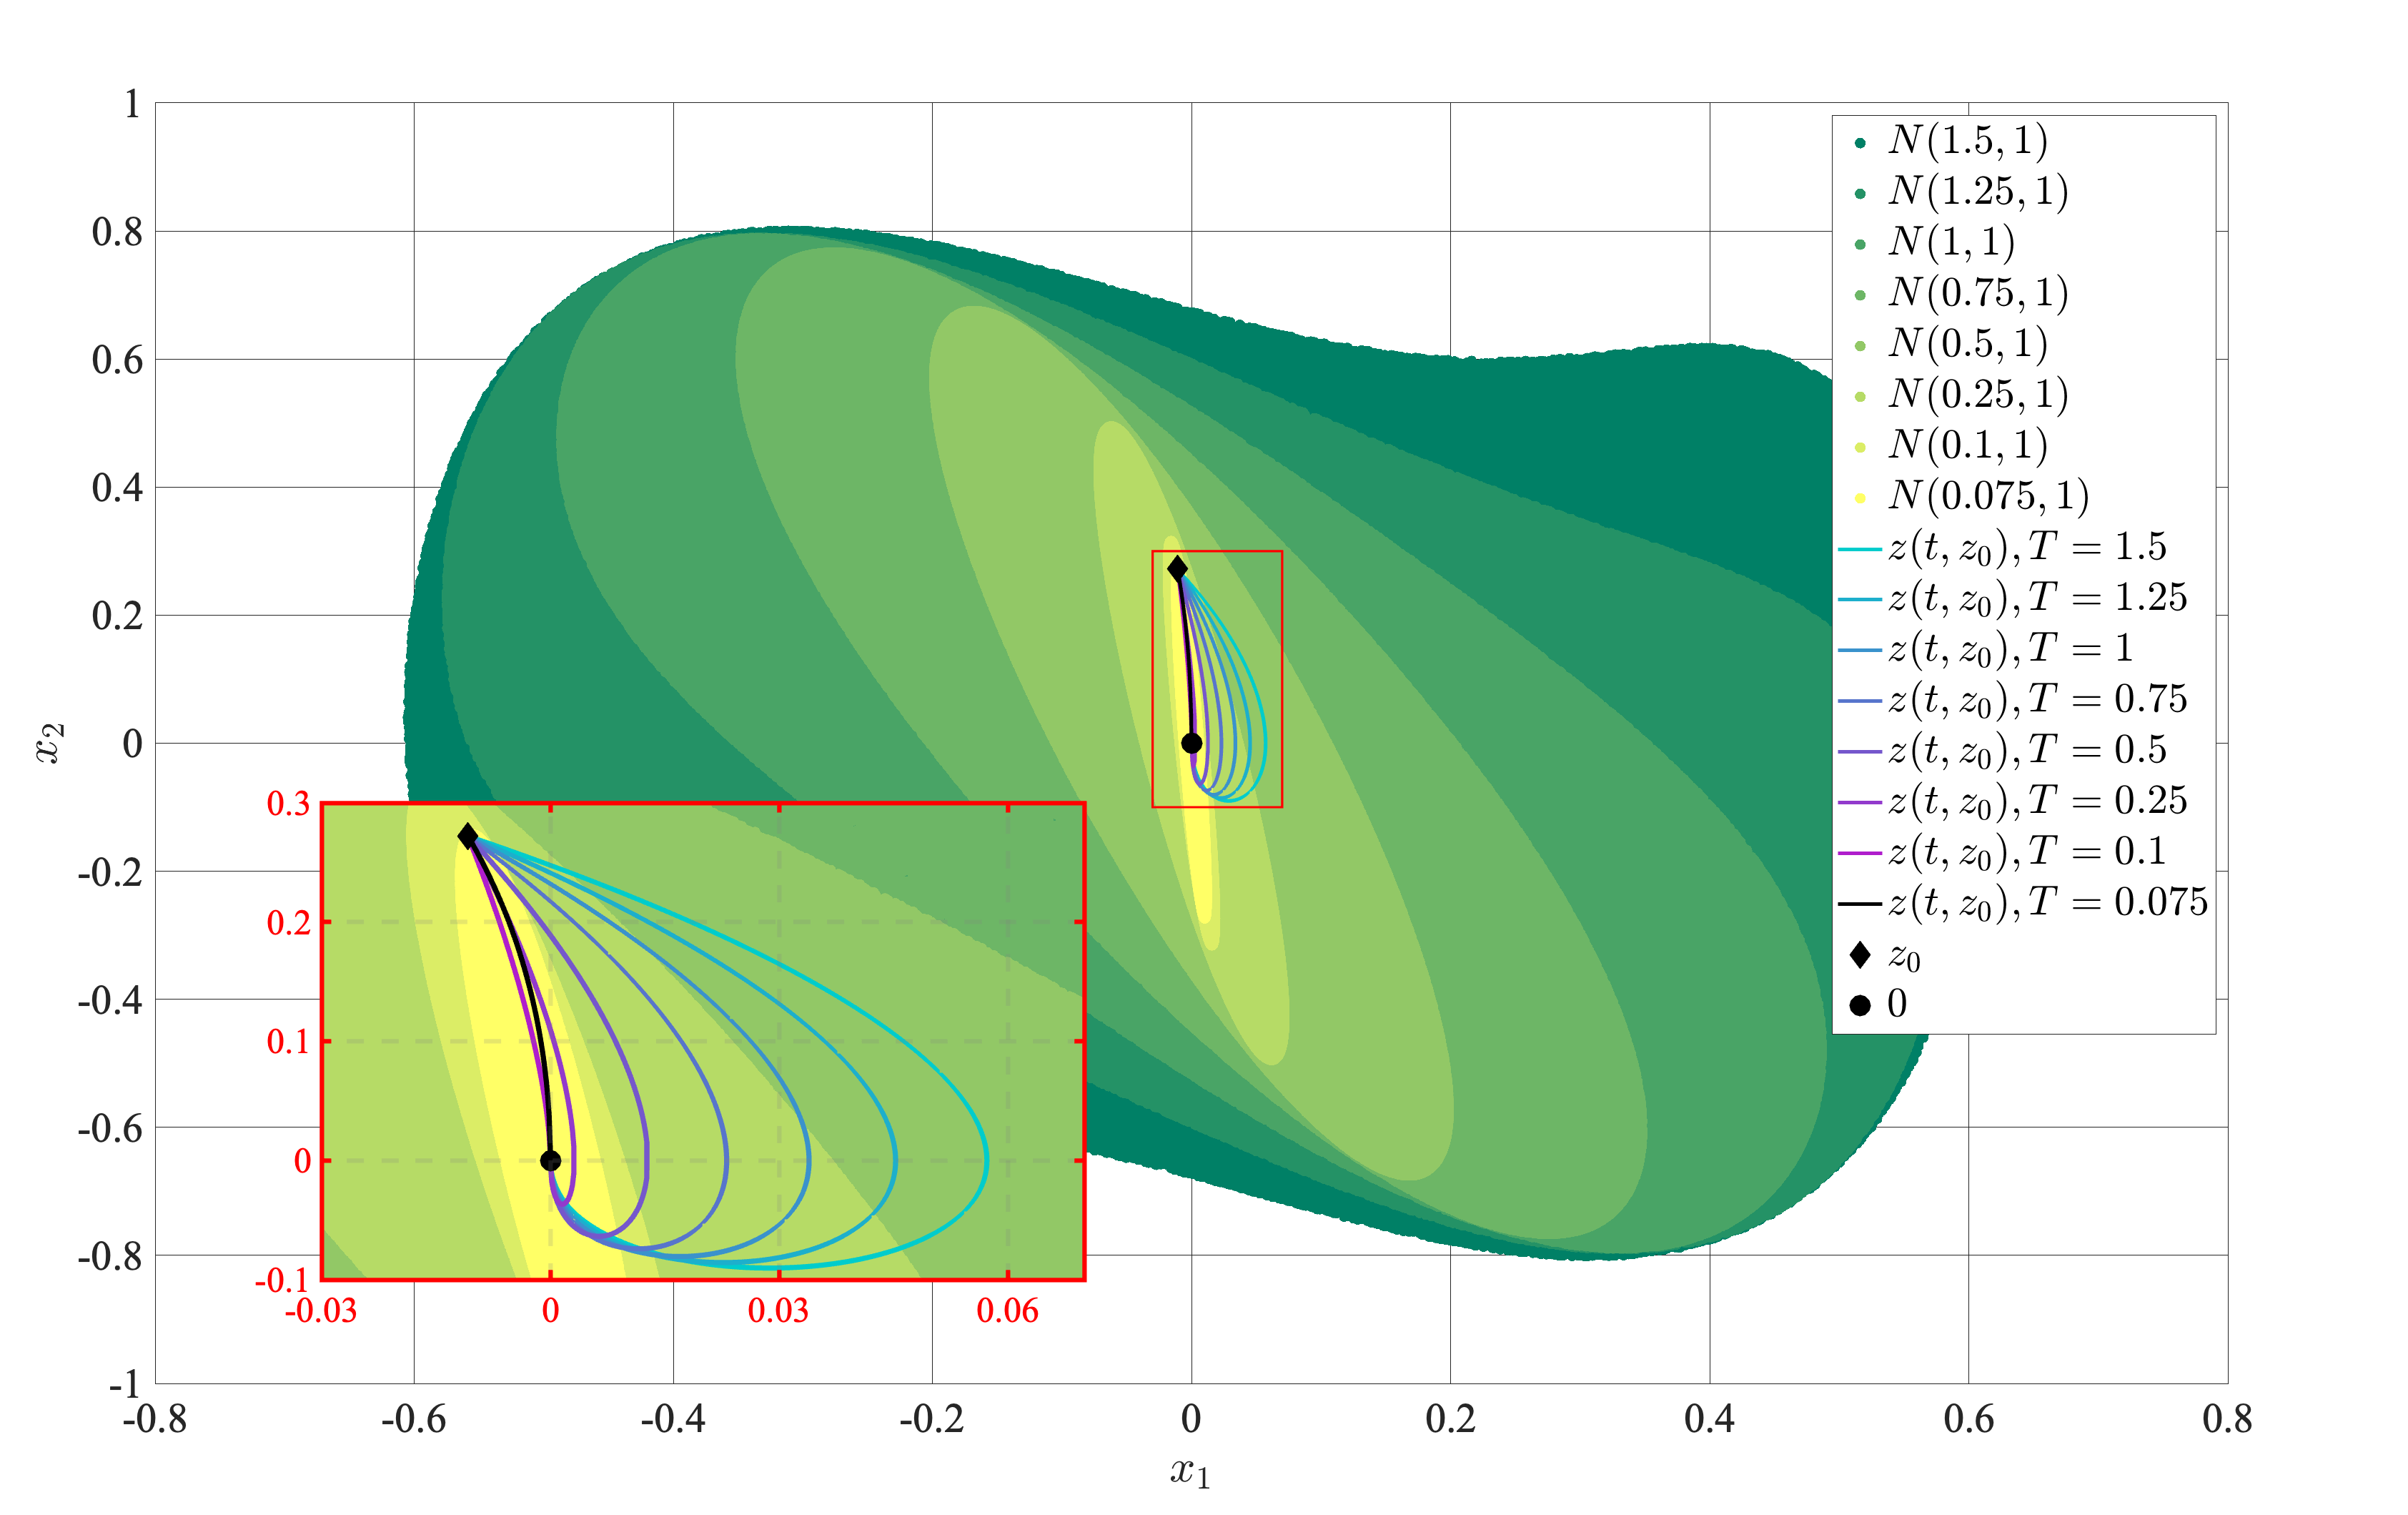
\includegraphics[width=\linewidth]{images/GusevMIOsipov_Duffing_fixed_z0.eps}
    \caption{Results of experiments with variable $T$.}
    \label{fig:series1}
\end{figure}

Despite the fact that condition $z_0 \in B(0,r_1(T))$ of Theorem \ref{th:tends_to_zero} is not satisfied with $r_1(T)$ used in the proof, the trajectories still tend to zero. This can be explained by a too strict choice of $r_1(T)$ and by the fact that Theorem \ref{th:tends_to_zero} only formulates sufficient conditions for trajectories to tend to zero. One can observe that in the case of fixed initial conditions, as $T$ decreases, the relative difference of the functionals $\Delta_J$ decreases, as follows from the estimate obtained in the theorem \ref{th:functional_error_estimate}.

Now we will change the conditions of the experiment quite a bit. We will change not only $T$ but also 
the initial conditions $z_0$ so that, firstly, the equality 
$z_0^{\top} Q_T(0) z_0 = 1$, and second, so that the point $z_0$ is inside 
the corresponding null-controllable set $G_{-}(T,1)$.


\begin{table}
\caption{Results of experiments with variable $T$ and $z_0$}
\label{ExampleTable2}
\begin{center}
\begin{tabular}{c|c|c|c|c|c|c}
     № &    $T$  & $z_0$            & $\|z_0\|^2$&$z_0^{\top} Q_T(0) z_0$ &$J(T,z_0)$&$\Delta_J$ \\ \hline 
     1 &   1.500 & [-0.594;-0.057]  & 0.356680   & 0.999993    & 1.075833 & 0.0758407 \\ \hline
     2 &   1.250 & [-0.578;0.226]   & 0.385032   & 0.999997    & 1.110464 & 0.1104671 \\ \hline
     3 &   1.000 & [-0.502;0.508]   & 0.509514   & 0.999999    & 1.108159 & 0.1081607 \\ \hline
     4 &   0.750 & [-0.354;0.652]   & 0.550391   & 1.000000    & 1.048784 & 0.0487844 \\ \hline
     5 &   0.500 & [-0.195;0.638]   & 0.445513   & 1.000000    & 1.009848 & 0.0098475 \\ \hline
     6 &   0.250 & [-0.069;0.481]   & 0.236487   & 1.000000    & 1.000349 & 0.0003490 \\ \hline
\end{tabular}
\end{center}
\end{table} 

The results of this series of experiments 
are shown in figure \ref{fig:series2} and in table 
\ref{ExampleTable2}. The notations are generally similar to figure \ref{fig:series1}: 
The green areas denote the null-controllable sets $G_{-}(T,1)$ of the system 
\eqref{Duffing} at $T = \{0.25, 0.5, 0.75, 1.0, 1.25, 1.5\}$, the dashed lines 
lines show the boundaries of the null-controllable sets of the linearized system 
\eqref{LinearDuffing}, the solid lines show the trajectories of the non-linear system 
at different $T$. The symbols "$\blacklozenge$" in different colours represent 
initial conditions $z_0$, and "$\bullet$" --- the target point located at 
at the origin. 

The remark about not fulfilling the condition from the first part of the example is also relevant here. Table \ref{ExampleTable2} shows that the values of $\Delta_J$ also decrease with decreasing $T$, but the decrease is not monotonic. This appears to be due to the fact that not only $T$ but also $z_0$ is changing. 

\begin{figure}
    \centering
    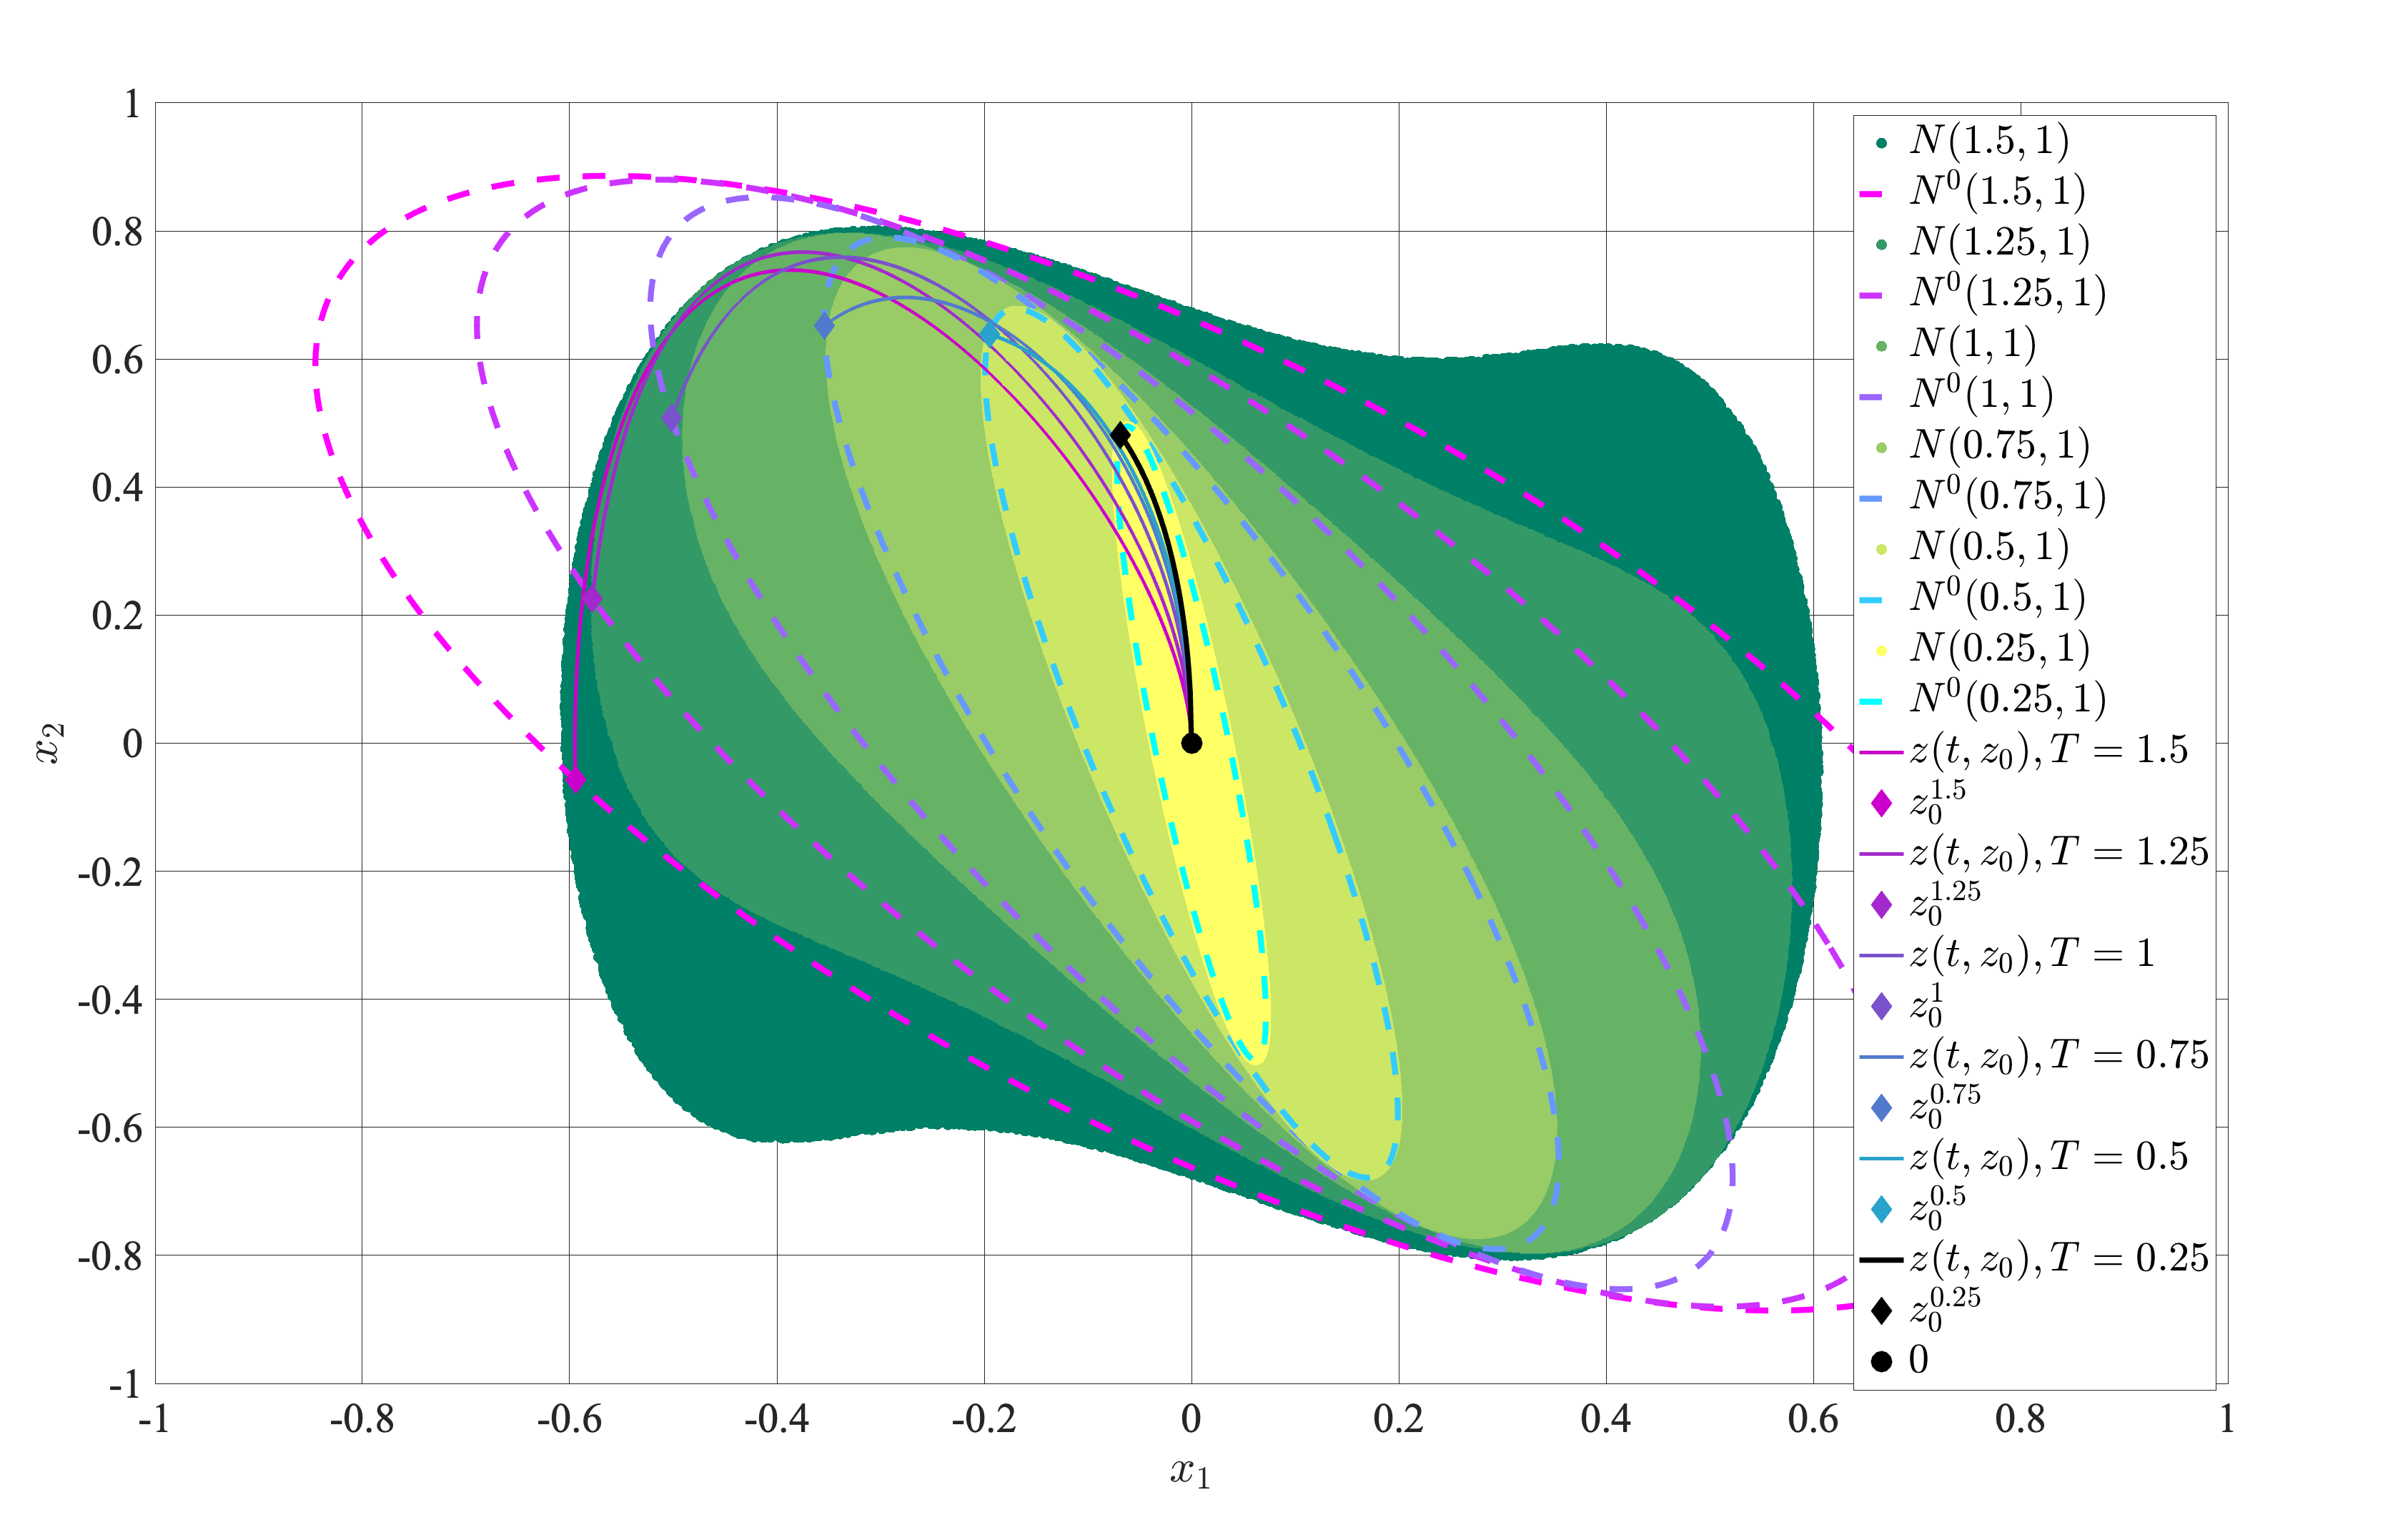
\includegraphics[width=\linewidth]{images/GusevMIOsipov_Duffing_variable_z0.eps}
    \caption{Results of experiments with variable $T$ and $z_0$.}
    \label{fig:series2}
\end{figure}

Also, in figure \ref{fig:series2} we can observe that the null-controllable sets of the nonlinear and linearized systems are close in form at $ T \leqslant 0.75$. 

\subsubsection{Conclusion}
It is shown that the linearization method may be applied
to the problem of an optimal control synthesis on a finite time interval. The  linear feedback controller, designed for the linearized  system, also provides a local solution to synthesis problem  for the nonlinear system if the interval is sufficiently small.  This requires fairly strict restrictions on the   controllability Gramian asymptotics, which  coincide with sufficient conditions ensuring the asymptotic equivalence of reachable  (null-controllable) sets. Under these conditions the estimate for the relative error  values of an integral cost was given. We used an example of a nonlinear spring system under the influence of an external force to demonstrate the implementation of the described synthesis method. 


\end{document}